

\documentclass{acm_proc_article-sp}
\usepackage{float}% If comment this, figure moves to Page 2
\usepackage{epstopdf}
\usepackage{pstricks}
\usepackage{graphicx}
\usepackage{placeins} 
\begin{document}

%\title{A Sample {\ttlit ACM} SIG Proceedings Paper in LaTeX
%Format\titlenote{(Does NOT produce the permission block, copyright information nor page numbering). For %use with ACM\_PROC\_ARTICLE-SP.CLS. Supported by ACM.}}
\title{GPSInsights: An efficient framework to manage and process masssive GPS vehicle data}

\subtitle{[Extended Abstract]
%\titlenote{A full version of this paper is available as
%\textit{Author's Guide to Preparing ACM SIG Proceedings Using
%\LaTeX$2_\epsilon$\ and BibTeX} at
%\texttt{www.acm.org/eaddress.htm}}
}
%
% You need the command \numberofauthors to handle the 'placement
% and alignment' of the authors beneath the title.
%
% For aesthetic reasons, we recommend 'three authors at a time'
% i.e. three 'name/affiliation blocks' be placed beneath the title.
%
% NOTE: You are NOT restricted in how many 'rows' of
% "name/affiliations" may appear. We just ask that you restrict
% the number of 'columns' to three.
%
% Because of the available 'opening page real-estate'
% we ask you to refrain from putting more than six authors
% (two rows with three columns) beneath the article title.
% More than six makes the first-page appear very cluttered indeed.
%
% Use the \alignauthor commands to handle the names
% and affiliations for an 'aesthetic maximum' of six authors.
% Add names, affiliations, addresses for
% the seventh etc. author(s) as the argument for the
% \additionalauthors command.
% These 'additional authors' will be output/set for you
% without further effort on your part as the last section in
% the body of your article BEFORE References or any Appendices.

\numberofauthors{8} %  in this sample file, there are a *total*
% of EIGHT authors. SIX appear on the 'first-page' (for formatting
% reasons) and the remaining two appear in the \additionalauthors section.
%
\author{
% You can go ahead and credit any number of authors here,
% e.g. one 'row of three' or two rows (consisting of one row of three
% and a second row of one, two or three).
%
% The command \alignauthor (no curly braces needed) should
% precede each author name, affiliation/snail-mail address and
% e-mail address. Additionally, tag each line of
% affiliation/address with \affaddr, and tag the
% e-mail address with \email.
%
% 1st. author
\alignauthor
Tobin%\titlenote{Dr.~Trovato insisted his name be first.}\\
       \affaddr{Institute for Clarity in Documentation}\\
       \affaddr{1932 Wallamaloo Lane}\\
       \affaddr{Wallamaloo, New Zealand}\\
       \email{trovato@corporation.com}
% 2nd. author
\alignauthor
G.K.M. Tobin%\titlenote{The secretary disavows
%any knowledge of this author's actions.}\\
       \affaddr{Institute for Clarity in Documentation}\\
       \affaddr{P.O. Box 1212}\\
       \affaddr{Dublin, Ohio 43017-6221}\\
       \email{webmaster@marysville-ohio.com}
% 3rd. author
\alignauthor Lars Th{\o}rv{\"a}ld%\titlenote{This author is the
%one who did all the really hard work.}\\
       \affaddr{The Th{\o}rv{\"a}ld Group}\\
       \affaddr{1 Th{\o}rv{\"a}ld Circle}\\
       \affaddr{Hekla, Iceland}\\
       \email{larst@affiliation.org}
}
% There's nothing stopping you putting the seventh, eighth, etc.
% author on the opening page (as the 'third row') but we ask,
% for aesthetic reasons that you place these 'additional authors'
% in the \additional authors block, viz.
\additionalauthors{Additional authors: John Smith (The Th{\o}rv{\"a}ld Group,
email: {\texttt{jsmith@affiliation.org}}) and Julius P.~Kumquat
(The Kumquat Consortium, email: {\texttt{jpkumquat@consortium.net}}).}
\date{30 July 1999}
% Just remember to make sure that the TOTAL number of authors
% is the number that will appear on the first page PLUS the
% number that will appear in the \additionalauthors section.

\maketitle
\begin{abstract}
Intelligent Transport System~(ITS) has seen growing interest in collecting various types of location-based data of transport vehicles in circulation in order to build up high quality real-time traffic monitoring system. Managing those massive data faces BigData challenges. In this paper we propose GPSInsights, a framework that can manage and process massive GPS vehicle data effectively. GPSInsights is built on scalable distributed, open-source software with Geomesa performing the key part.  We demonstrate our framework with a scalable map matching implementation and perform experiments with big dataset. 

% A category with the (minimum) three required fields
\category{H.4}{Information Systems Applications}{Miscellaneous}
%A category including the fourth, optional field follows...
\category{D.2.8}{Software Engineering}{Metrics}[complexity measures, performance measures]

\terms{Bigdata}

\keywords{GPSInsights, spatio-temporal data storage, distributed data processing, map matching}
\end{abstract}

\section{Introduction}


With the widespread adoption of GPS technology, Intelligent Transport System~(ITS) has seen growing interest in collecting various types of location-based data of transport vehicles in circulation. This data collection is done with the purpose of being able to deliver not only high quality real-time traffic monitoring but also useful traffic statistics and predictive information. Lee et al.~\cite{Lee2011} a data mining algorithm to discover traffic bottlenecks. Demiryurek et al.~\cite{Demiryurek2010} proposed an online computation of optimal traffic route based on traffic data. 
	
According to Decree No. 91/2009/ND-CP of Ministry of Transport of Vietnam, all Vietnamese-licensed cars in must be equipped with a standardised GPS monitoring system (black-box) which reports geo-location, speed and direction every 30 seconds to a centralised data centre. With nearly 200.000 cars in circulation in the near future, those collecting data are enormous and have characteristics of BigData. The first characteristic is big volume that refers to the increasing amount of data (petabytes) need to be stored with a relatively low cost. The second characteristic is big velocity that refers to the data generation speed, at which the underlying system must deliver. The third characteristic is big value because mining those data gives insights about the current situation of the traffic infrastructure, as well as, the predictions. 

As BigData create non-conventional challenges, current ITS management systems storing data in relational database system (e.g. via PostGIS) will not be able to adapt to the data ingestion speed, nor being able to be mined efficiently. In this work, we describe GPSInsights: a novel scalable system for manipulating and processing GPS traffic data. First, GPSInsights is able to handle big volume of data at the level of petabytes efficiently in distributed environments. Second, GPSInsights deals with big velocity where millions of GPS messages coming from millions of cars in Vietnam are ingesting into the system every 30 seconds. Third, despite big volume and big velocity challenges, GPSInsights can deliver in-time analytic reports for good uses. We demonstrates GPSInsights with a scalable map matching implementation. 

This paper is organised in 7 parts. In Section 2, we discuss an overall architecture of our system framework. In Section~3, we go into the details of the technologies and components of GPSInsights. In Section~4, we establish a simple demonstration map matching algorithm. Section~5 presents experimental results for the algorithm presented in Section~4. Section~6 discusses related works on existed map matching algorithms and on storing spatio-time data. We conclude and discuss future work in Section~7.
	
\section{The general system design} 
	
After being sent continuously from moving vehicles to converging data centers (note), the transportation information data will be pulled into a data mining block. The data mining block will process, analyze them and then send statistic results to a visual display system through a connect module. The general system design is illustrated as follow:

\begin{figure}[!htb]
\centering
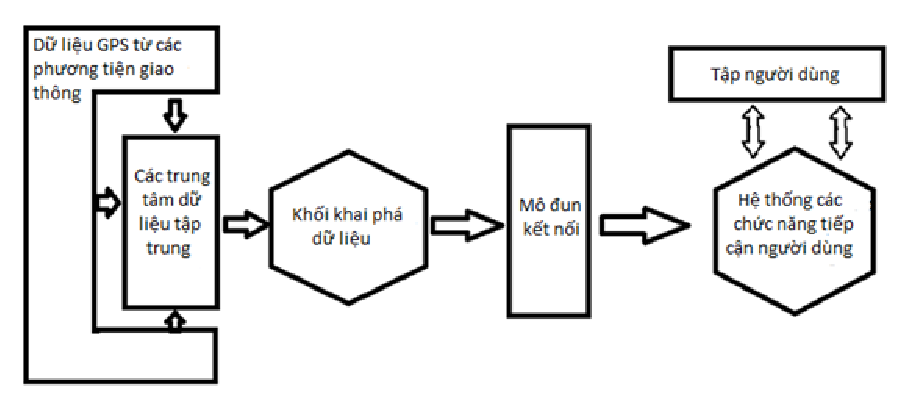
\epsfig{file=thesis-1.eps, height=140px, width=250px}
\caption{The architecture of the system}
\end{figure}

As a massive amount of transportation data being directed to these centers per second, the data mining block has to have following requirements.
-	The collected data are put in their order of arrival in time, and all of them have to be processed at least one.
-	The processing time is acceptable. With a quantity of data, the processing time  must not exceed than the collecting one.
-	Final statistic results have to be saved for using later.

In order to meet with the above requirements and deal with the challenges of big volume, velocity, it is necessary to construct the data mining block as a scalable system with scalable components as follows.

-	Message queue: As the transportation information data come continuously from a variety of sources,  this component are supposed to combine the multi-source data, and put them in their order of arrival in time. In addition, it has to store and replicate the large input data dispersedly on a large cluster for high-throughput, fault-tolerance.

-	Data processing engine: After storing the input data persistently, we also need a engine that has the ability to process them fast and continuous. A distributed, parallel and continuous processing engine totally meet this need.

-	Result queue: Results from data processing engine are sent to this component before being moved to the connect module. This component has to have the ability to write and read a massive amount of data in short time. The purpose of these is to reduce the waiting time of the data processing engine when pushing the final statistic results to the connect module.

-	Result storage: The result storage is used to store the big-volume and high-velocity statistic results from the data processing engine. Hence, we need a distributed data storage. It also has the ability to write data fast in order to avoid increasing the processing time of the data processing engine. 

One another reason of choosing the message queue as a component of the data mining block is an increase in the fault-tolerance for the block. In the case the transportation data are sent directly to the data processing engine, if its the master node crashes, it will stop working. So all data come in that time will disappear.



\section{Implementation} 

With the system architecture shown in section 2, we have decided to build a system based on components which are described as below, and we will explain the reasons for choosing the components and how they interact with each other.

\begin{figure}[!htb]
\centering
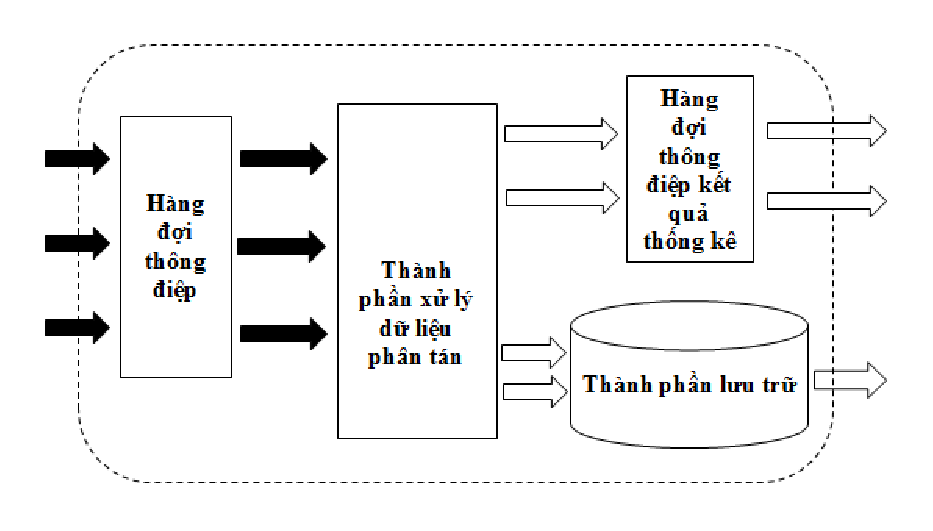
\epsfig{file=thesis-2.eps, height=125px, width=250px}
\caption{The architecture of the system}
\end{figure}

\textbf{Message queue: Apache Kafka.} Apache Kafka is the distributed publish-subscribe messaging. Kafka stores the data in categories called topic. A topic will be divided into one or more partitions which be distributed over nodes of a cluster (each partition is an ordered, immutable sequence of messages). It allows store the amount of the data larger than the capability of any single machine.
Reading to and writing data in topic are very fast, thanks to paralleling operations and several useful techniques installed to maximize the performance (http://www.slideshare.net/baniuyao/kafka-24299168). According to Kafka's official website, a single Kafka broker can handle hundreds of megabytes of reads and writes per second from thousands of clients.
Kafka also is designed to allow transparently and easily expanded without downtime. In addition, partitions are persisted on disk and replicated within the cluster to prevent data loss. So Kafka offers strong scalable, durability and  fault-tolerance.

\textbf{Data processing engine: Spark Streaming.} Spark Streaming is a module of Apache Spark for acting on data stream as soon as it arrives. It provides an abstraction called Dstreams (discretized streams). A Dstream is represented as a continuous sequence of data arriving over time. In a more detail, a set of data arriving at each time step will be packed in a batch called an RDD, so each Dstream is a continuous sequence of RDDs. An RDD is simply an immutable distributed collection of objects. We can not change any property of an object in RDD. Using Map-Reduce model, Each RDD is split into multiple partitions, which may be processed on different nodes of a cluster. Every operations on partitions of RDD also are executed in memory, so running programs on Spark Streaming is very fast. According to Spark's official website, by comparison with the time of executing a logistic regression in Hadoop, running time in Spark is 100 times faster.
Spark's RDDs also offer a strong fault-tolerance , because the input data are replicated to another nodes of the cluster, and an RDD remembers the lineage of deterministic operations that were used on that data to create it. If any partition of an RDD is lost due to a node failure, as long as a copy of the input data is still available, then that partition can be re-computed from it using the lineage of operations.



\section{Demonstration: Scalable map matching}
\subsection{Dataset}
Our data include about 12,565,521 GPS records collected by vehicles equipped with a GPS receiver from 22/03/2014 to 22/04/2014 in Ho Chi Minh city. Every record consists of speed, GPS coordinate and state of the vehicle and the period of time between two records is 15 minutes. The following table shows the format of the data.

\begin{table}[h]
\centering
\begin{tabular}{|c|c|c|c|c|}
\hline
\textbf{time\_stamp} & \textbf{car\_id} & \textbf{lon}   & \textbf{lat} & \textbf{speed} \\ \hline
\end{tabular}
\end{table}

\subsection{Algorithm: Road Reverse Geocode Algorithm Using K-D Tree.}	
	
\subsubsection{Process OSM raw data.}
	The Open Street Map's raw data consist of a mass of tag almost covering the whole world. Every node tag has some tags inside to determine its attributes (e.g. type, way's name, coordinate, ..). Way tag contains one or more node tags that used to define the shape of it.
	
		\setlength{\parindent}{0.7cm} Before going to the details, vertices, links and segments should be defined clearly. Link is a section of road between intersections. In most digital maps, a real road is digitized and is described with a set of many straight lines. Vertices are points which separate these straight lines, and each straight line is a segment. The road AD in Fig.~\ref{fig:composition} is formed by 3 intersections (black points), 2 vertices (white points), 2 links (AD, DE) and 3 segments(AB, BC, CD).
		
\begin{figure}[h]
\centering
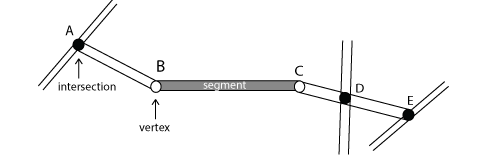
\includegraphics[height=100px,width=210px]{figure1}
\caption{The composition of the road network}
\label{fig:composition}
\end{figure}
	
		\setlength{\parindent}{0.7cm} Our purpose is to determine all links and their information (name of roads which contain these links). Firstly, we traverse the tag list of OSM, read all Way tags, ignore irrelevant ways (roads that are unfit for transports such as cars, taxis and buses) and then store all associated node ids (we use BTree for this task). If a node occurs once, it is a vertex. Otherwise, it is an intersection. Secondly, we store all Node tags for later uses.
	
\subsubsection{Link matching.}
	
	Because the transport data are collected from GPS tracking device, the input consists of a sequence which contains a time stamp and a geographic coordinate. Our task is to assign a GPS point to a relevant link. Kd-tree is chosen to tackle this problem~\cite{moh2013approximate}. It is an efficient searching method to quickly find nearest points and this algorithm only takes O(log n) average time per search in a reasonable model.
	
	\setlength{\parindent}{0.7cm} Despite the fact that the standard deviation of GPS data could be quite low in the best case, around 3 meters, it can increase several fold due to tree cover, tunnel and other problems. The limited sampling polling time intervals is the second source affecting the accuracy. There are many methods to solve quite effectively this, including vertex-based and segment-based map matching, map matching using the geometric relationship, map matching using the network topology, the data history and so forth. This paper does not focus on this problem, we only use the vertex-based map matching for the simplicity of the process.  
	
%	\begin{figure}
%		\subfloat[vertex-based map matching]{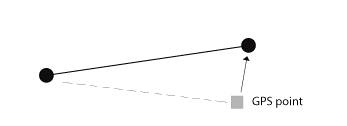
\includegraphics[width = 0.5\linewidth]{figure3}} 
%		\subfloat[Add some equidistant vertices in segments]{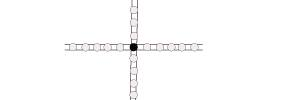
\includegraphics[width = 0.5\linewidth]{figure2}\label{fig:sfig2}}
%	\caption{Link matching}
%	\end{figure}
	
	\setlength{\parindent}{0.7cm} We go through the list of ways in OSM and add some equidistant vertices in segments ( illustrated in Fig.~\ref{fig:sfig2}) and build a KD-Tree based on those vertices. Note that a node in the Kd-Tree consists of a coordinate and information of a link which associates it. Therefore, by taking a GPS point into the Kd-Tree and using the vertex-based map matching, we can determine its nearest vertex as well as a link it is matched to.
	
	\subsubsection{Describe our algorithm.}
		
	\setlength{\parindent}{0.7cm} In this section, we focus on explaining our proposed algorithm in traffic volume statistic. With this algorithm, we query vehicle object q in a specific time period and a GPS bound from Geomesa aimed at achieving following attributes of q: q's latitude, q's longitude and q's speed. All the information we will store in a data structure list – input. After getting input data from Geomesa, now, we review how Spark is used in our algorithm. Firstly, we build up a kdTree with OSM data preprocessed and then broadcast it to the nodes in our system (Line 14). By doing this, we can keep a read-only variable cached on each machine instead of shipping a copy of it with tasks, thereby, providing every node a copy of the kdTree which make up a lot of memory and construction time. Secondly, it is necessary for our algorithm to utilize a collection in-parallel in order to construct a distributed dataset from input data list which can be operated on in paralle. Because the parallel collection can be used many times, we will cache it on memory accelerating our program (Line 15).
	
\setlength{\parindent}{0.7cm} As we have a parallelized collection formed, our algorithm will be divided into two phase: a data mapping phase and a data collecting phase. 

\subsubsection{Data Mapping Phase:} All the elements of the parallelized collection (object q) will be passed on the maptopair method of spark which can operate on in-parallel. As every object q go into the method, the nearestPoint method of copies of kdTree cached on each machine can be utilized aimed at finding what point of a road segment (p) is nearest point of object q and how long distance between q and p (Line 19). Because of the fact that coordination GPS sent from satellites will have some deviations in comparison with the real coordinate, so that we have to choose a threshold distance in order to determine whether object q belong to the road segment including p or not (Line 20 - 27). If the distance is smaller than the threshold distance, it will be much easier for us to conclude that the object q belongs to the road segment and vice versa. As a result, our algorithm can remove the object q that its distance with the road segment is too far from, therefore, we can enhance the accuracy of our algorithm to some extent. Finally, in the Line 29, after every object q is matched to a road segment by road segment's ID, we will group the matched pairs by road segment's ID, hence, we can obtain $<$key, value$>$ pairs with key being a roadID and value being a iterable of vehicleID and speed.

\setlength{\parindent}{0.7cm} In the next step in the phase, we will continue to process the $<$key, value$>$ pairs in-parallel by using the maptopair method of spark. The number of vehicle moving on a road segment also the average speed of the road segment will be calculated in the step (Line 33 - 34).

\subsubsection{Data Collecting Phase:} In data mapping phase, statistic numbers of the road segments will be processed in-parallel on the nodes of our system, so that collecting the data perform a decisive role in our algorithm. After the figures are processed, we will use the collect method of spark to convert the parallel collection into a simple list in order to summarize the information and, therefore, we will achieve statistic numbers of traffic volume and average speed on each road segments (Line 38 - 40).


{\it The Pseudocode of Algorithm}	
\begin{verbatim}

\end{verbatim}
%
\noindent

\section{Experimental Evaluation}
	Our system set up on a cluster of HPCC super computer which has one master node and three compute nodes . The configuration of each node include an Intel Xeon E5-2670 Processor (20M Cache, 2.6 GHz, 8 Core), 32 GB DDR3 RAM and FDR 56Gbps Infiniband.
	
	With this configuration, we have conducted several experiments on our data set shown in section 4.1 aimed at appreciating execution time and performance of the architecture. After querying data from Geomesa according year, month, day of month and hour of day and removing records that its speed attribute is 0, we obtained 1,200,000 records. We compared the running time of the system on the whole records and the half records with various numbers of nodes. The result is illustrated by Figure 6.
	
	% 	 Suppermicro SC815TQ-600WB\\ Intel Xeon E5-2670 Processor (20M Cache, 2.6 GHz, 8 Core)\\	 32 GB DDR3 RAM\\	 2*250 GB HDD\\	 FDR 56Gbps Infiniband\\
	
	\begin{figure}
		\centering
		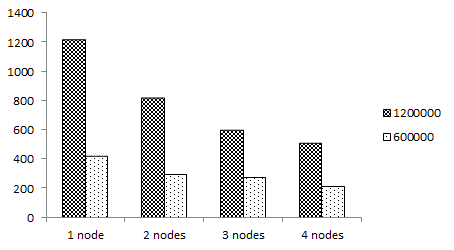
\includegraphics[height=150pt,width=200pt]{figure6}
		\caption{The execution time of the system}
	\end{figure}

\setlength{\parindent}{0.7cm} It is worth noting that as the figure for nodes was increased, the execution time of the system reduced steadily due to the parallel procedure of spark. While effective indexing strategy of Geomesa enable the architecture to quickly query data from Geomesa, spark help the algorithm to accelerate computation by processing in-parallel. As shown in Figure 6, similarity to 600,000 records, with 4 nodes established, the system take a few more than 500s for 1,200,000 records and less than halving of the running time of the system since we only run on 1 node - a considerable decrease. Besides, we installed a common system running without parallel and kind of indexing strategy like Geomesa such as: using Hash Map with normal database in order to have a comparison with our system. With 1,200,000 records, after 20,000s running, there was no signs of stopping of the system.
	
\section{Related work}

PostGIS~\cite{posgis} is a spatial database extender for PostgreeSQL object-relational database, adds support for geographic objects allowing location queries to run in SQl. Remember that the relational database has the ability to use information from multiple indexes to determine how best to search for the records that satisfy all query criteria, so it is good for multi-dimension data rather than a key-value store. It is undeniable that PostGis completely meets most of the spatial-temporal query and there are a large number of software products that can use PostGIS as a database backend~\cite{backendposgis}. However, spatio-temporal data sets have seen a rapid expansion in volume and velocity due to the rapid increase of means of transport and GPS device, which is about hundred millions and more records per day. With the reason that the capacity of a PostGIS is only about five hundred millions rows, we have to buy more hardware to meet the demand. However, we will have to cope with many issues such as data management, hardware cost and performance. It is clearly that Accumulo and Geomesa are good for tackle big transport data set.

There are a number of studies on matching GPS observations on a digital map. We can generally classify them into two categories~\cite{yang2005map} Map-matching algorithms using only geometric relationships between GPS data and a digital map and Map-matching consider not only geometric relationships but also the topology of the road network and history of GPS data.
		
		\setlength{\parindent}{0.7cm} Map-matching in first category can be classified by Noh and Kim(1998)~\cite{noh1998map} into the map matching algorithm using the distance of point-to-curve. One using the distance of curve-to-curve and one using the angle of curve-to-curve.
		
		\setlength{\parindent}{0.7cm} Map-matching using the network topology and the data history match the present point to a link based on the result of matching the previous point. However, when the distance between them is higher than a threshold then this method will use only the geometric relationships to match the GPS points to the nearest link.
		
		\setlength{\parindent}{0.7cm} Map-matching using the network topology and the data history are not appropriate for our GPS data which is described in the section~4. Neither of those two categories has demonstration with a scalable algorithm building with a distributed processing engine. 
			
	\section{Conclusion and Future Work}
	In this paper, we proposed an efficient framework to manage and process massive amount of GPS vehicle data. With the framework, we can conduct vehicle data statistics efficiently. Thus, we believe that GPSInsights can address an increasing number of the problem classes relating massive GPS vehicle data. We intend to pursue this framework in three directions. Firstly, we plan to use the framework in order to re-imitate routine of a vehicle with a dataset that the period of time between 2 times recording GPS coordinates is significant. Secondly, we research to use this framework for transport state prediction. And finally, the framework also can be used to build up the fastest path finding system.
			

%
% The following two commands are all you need in the
% initial runs of your .tex file to
% produce the bibliography for the citations in your paper.
\bibliographystyle{abbrv}
\bibliography{dasfaa2015}  % sigproc.bib is the name of the Bibliography in this case
% You must have a proper ".bib" file
%  and remember to run:
% latex bibtex latex latex
% to resolve all references
%
% ACM needs 'a single self-contained file'!
%
%APPENDICES are optional
%\balancecolumns
\appendix
%Appendix A
\section{Headings in Appendices}
The rules about hierarchical headings discussed above for
the body of the article are different in the appendices.
In the \textbf{appendix} environment, the command
\textbf{section} is used to
indicate the start of each Appendix, with alphabetic order
designation (i.e. the first is A, the second B, etc.) and
a title (if you include one).  So, if you need
hierarchical structure
\textit{within} an Appendix, start with \textbf{subsection} as the
highest level. Here is an outline of the body of this
document in Appendix-appropriate form:
\subsection{Introduction}
\subsection{The Body of the Paper}
\subsubsection{Type Changes and  Special Characters}
\subsubsection{Math Equations}
\paragraph{Inline (In-text) Equations}
\paragraph{Display Equations}
\subsubsection{Citations}
\subsubsection{Tables}
\subsubsection{Figures}
\subsubsection{Theorem-like Constructs}
\subsubsection*{A Caveat for the \TeX\ Expert}
\subsection{Conclusions}
\subsection{Acknowledgments}
\subsection{Additional Authors}
This section is inserted by \LaTeX; you do not insert it.
You just add the names and information in the
\texttt{{\char'134}additionalauthors} command at the start
of the document.
\subsection{References}
Generated by bibtex from your ~.bib file.  Run latex,
then bibtex, then latex twice (to resolve references)
to create the ~.bbl file.  Insert that ~.bbl file into
the .tex source file and comment out
the command \texttt{{\char'134}thebibliography}.
% This next section command marks the start of
% Appendix B, and does not continue the present hierarchy
\section{More Help for the Hardy}
The acm\_proc\_article-sp document class file itself is chock-full of succinct
and helpful comments.  If you consider yourself a moderately
experienced to expert user of \LaTeX, you may find reading
it useful but please remember not to change it.
\balancecolumns
% That's all folks!
\end{document}
